\documentclass[12pt]{article}
\setlength{\parskip}{2pt}%
\setlength{\parindent}{0pt}%
\usepackage{enumitem, amsmath, graphicx, wrapfig, float, nccmath, verbatim, fancyvrb, geometry, changepage}
\usepackage[export]{adjustbox}
\title{%
	ECE-471 Selected Topics in Machine Learning \\
	Prof. Curro \\
	Midterm Project}
\author{Evan Bubniak, Zhang Jinhan}
\begin{document}
\maketitle

\section{Results}

\begin{figure}[H]
	\centering
	\includegraphics[width=0.75\textwidth]{paper_source/fig.png}
	\caption{Juxtaposition of the noisy data points, the noiseless sinewave they are based on, and the manifold of the stochastic gradient descent regression model.}
\end{figure}

\begin{figure}[H]
	\centering
	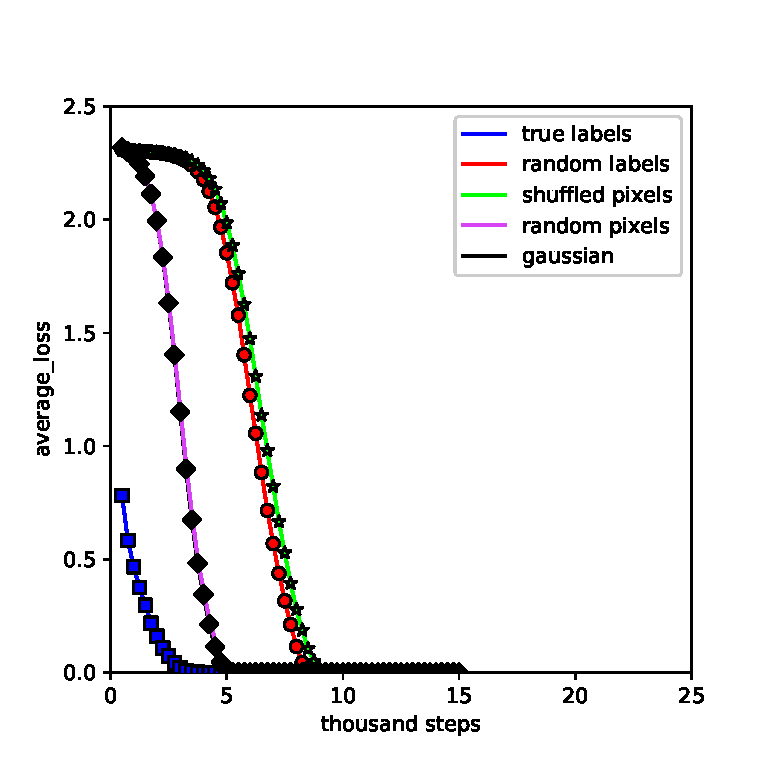
\includegraphics[width=0.75\textwidth]{results_1/output.eps}
	\caption{A plot of each of the basis functions, with the weights and intercept removed.}
\end{figure}

\clearpage
\begin{adjustwidth}{-50pt}{0pt}

\section{Code}

\end{adjustwidth}

\end{document}